\section{DCF Driver and Terminal-Value Audit}

Growth, reinvestment, WACC and terminal closure are shared across gold engines. Table~\ref{tab:dcf_inputs} summarizes the corporate assumptions.

\subsection{Growth, ROIC and reinvestment}
Growth and ROIC converge linearly to their stable levels over the five rate years since valuation. Reinvestment follows $b_t=g_t/ROIC_t$, linking growth to the capital required to sustain it (Figure~\ref{fig:dcf_driver_schedule}).

\noindent\begin{minipage}{\columnwidth}
{\centering
  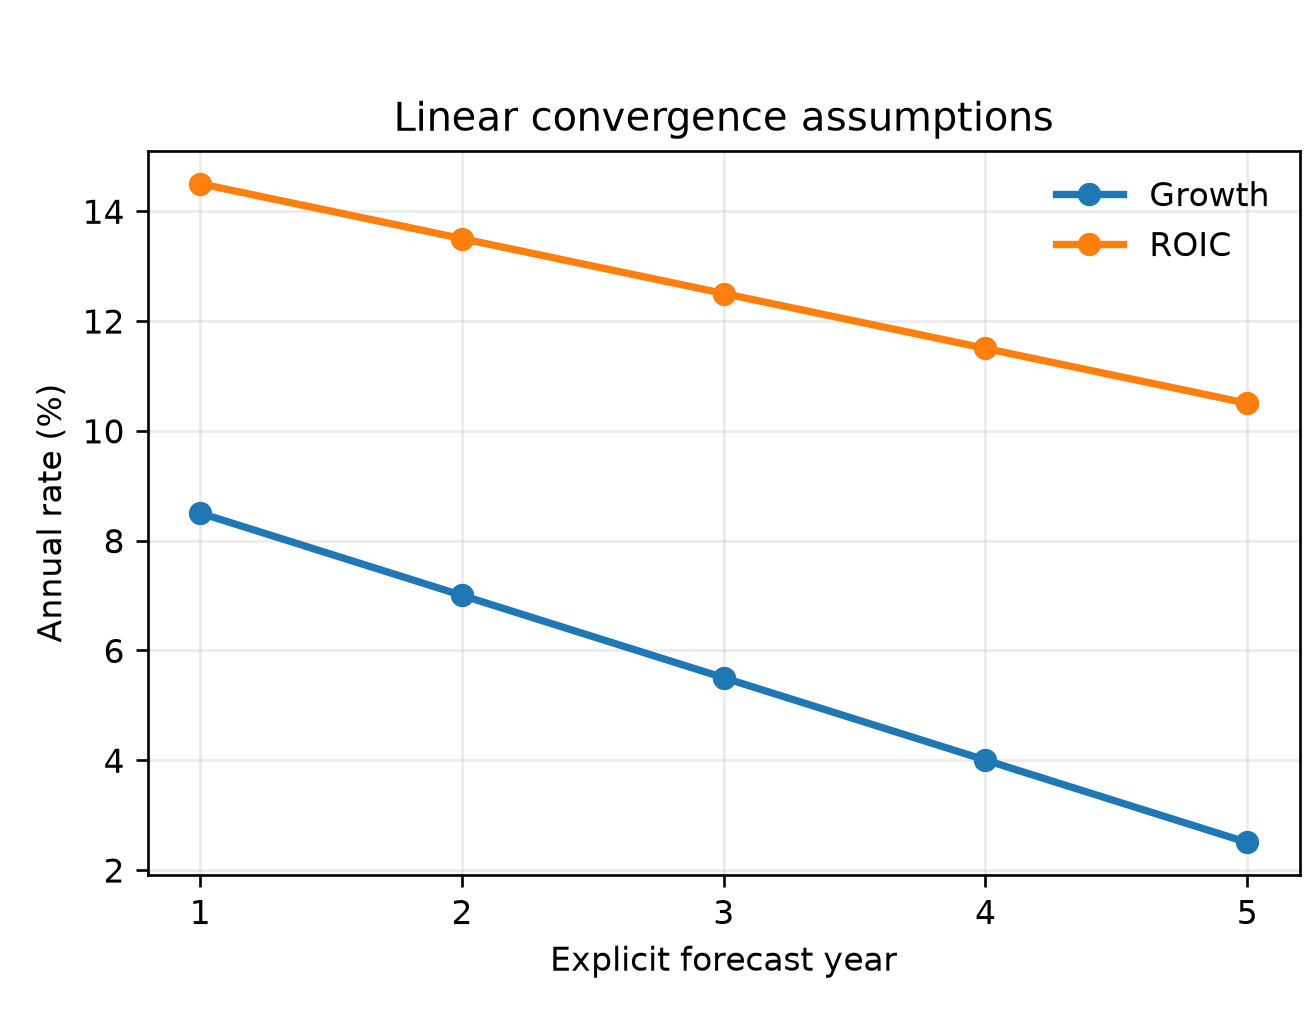
\includegraphics[width=0.90\linewidth]{../img/publication/ed4f022292eacd31_fig_dcf_growth_roic.png}
  \captionof{figure}{Common explicit-period DCF schedule: growth and ROIC converge linearly over the five-year horizon.}
  \label{fig:dcf_driver_schedule}
\par}
\end{minipage}\par

\noindent\begin{minipage}{\columnwidth}
{\centering
  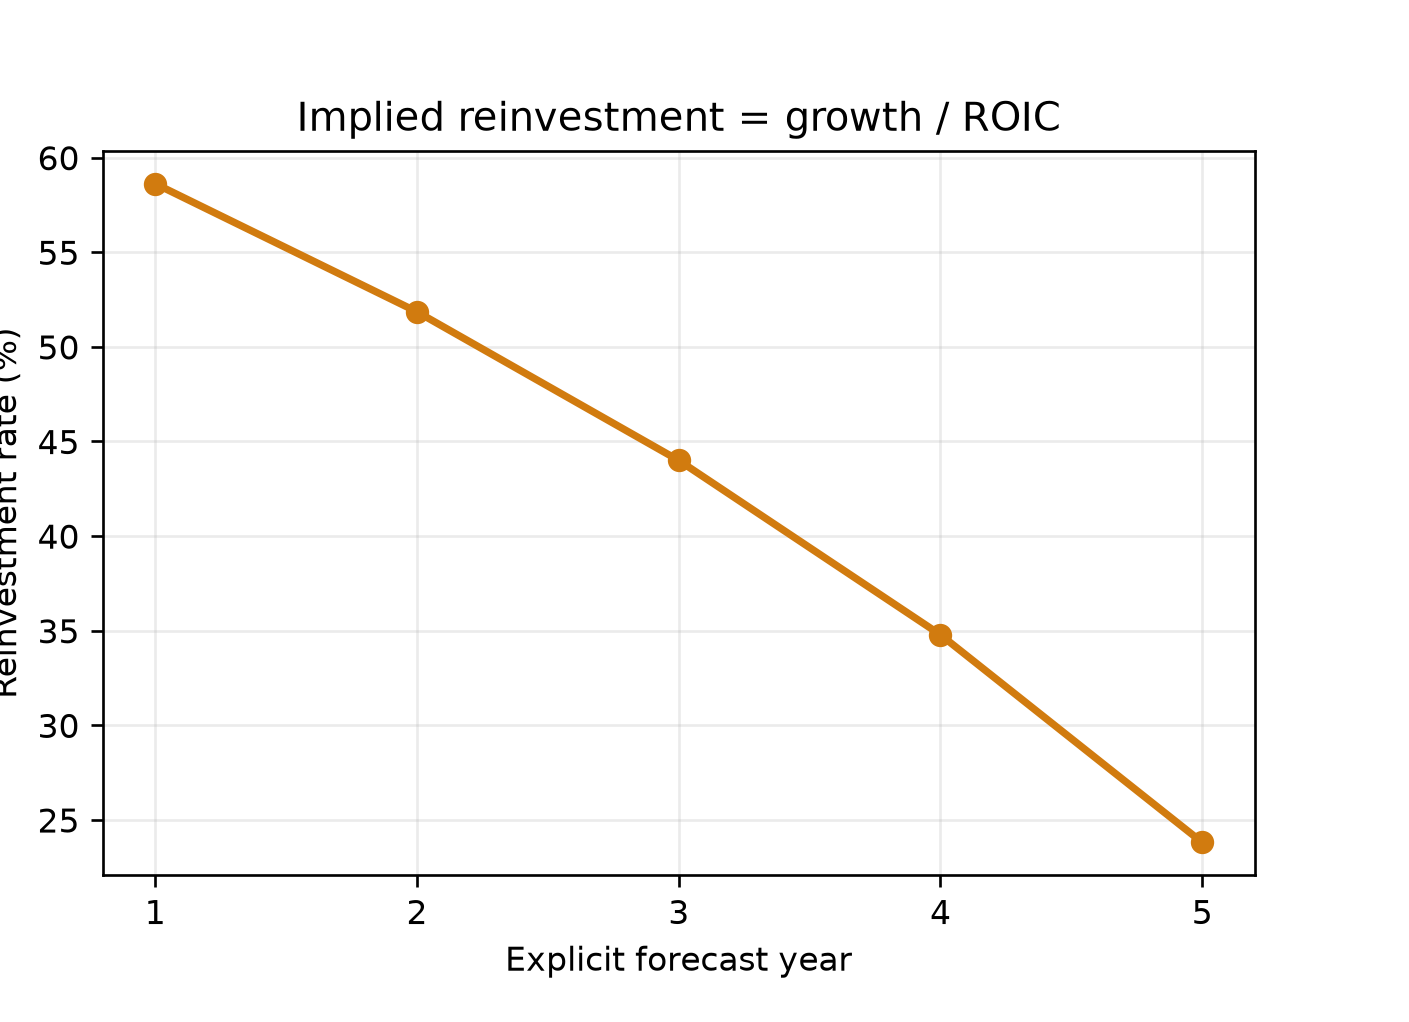
\includegraphics[width=0.90\linewidth]{../img/publication/ccbd1218e069545e_fig_dcf_reinvestment.png}
  \captionof*{figure}{\textbf{Figure~\ref{fig:dcf_driver_schedule} (continued).} The implied reinvestment rate, defined as growth divided by ROIC, falls from 58.62\% to 23.81\%.}
\par}
\end{minipage}\par

\subsection{Common stochastic WACC}
WACC follows the bounded mean-reverting process in Equation~\eqref{eq:wacc_process}, with inputs in Table~\ref{tab:dcf_inputs}; $w_0$ applies to the first year after valuation. Its annual innovation scale is $\sigma_w^*=\sigma_w\sqrt{(1-e^{-2\kappa_w})/(2\kappa_w)}=0.7308$ percentage points before clipping. All engines reuse the same 8,192 shock paths (Figure~\ref{fig:wacc_assumptions}).

\noindent\begin{minipage}{\columnwidth}
{\centering
  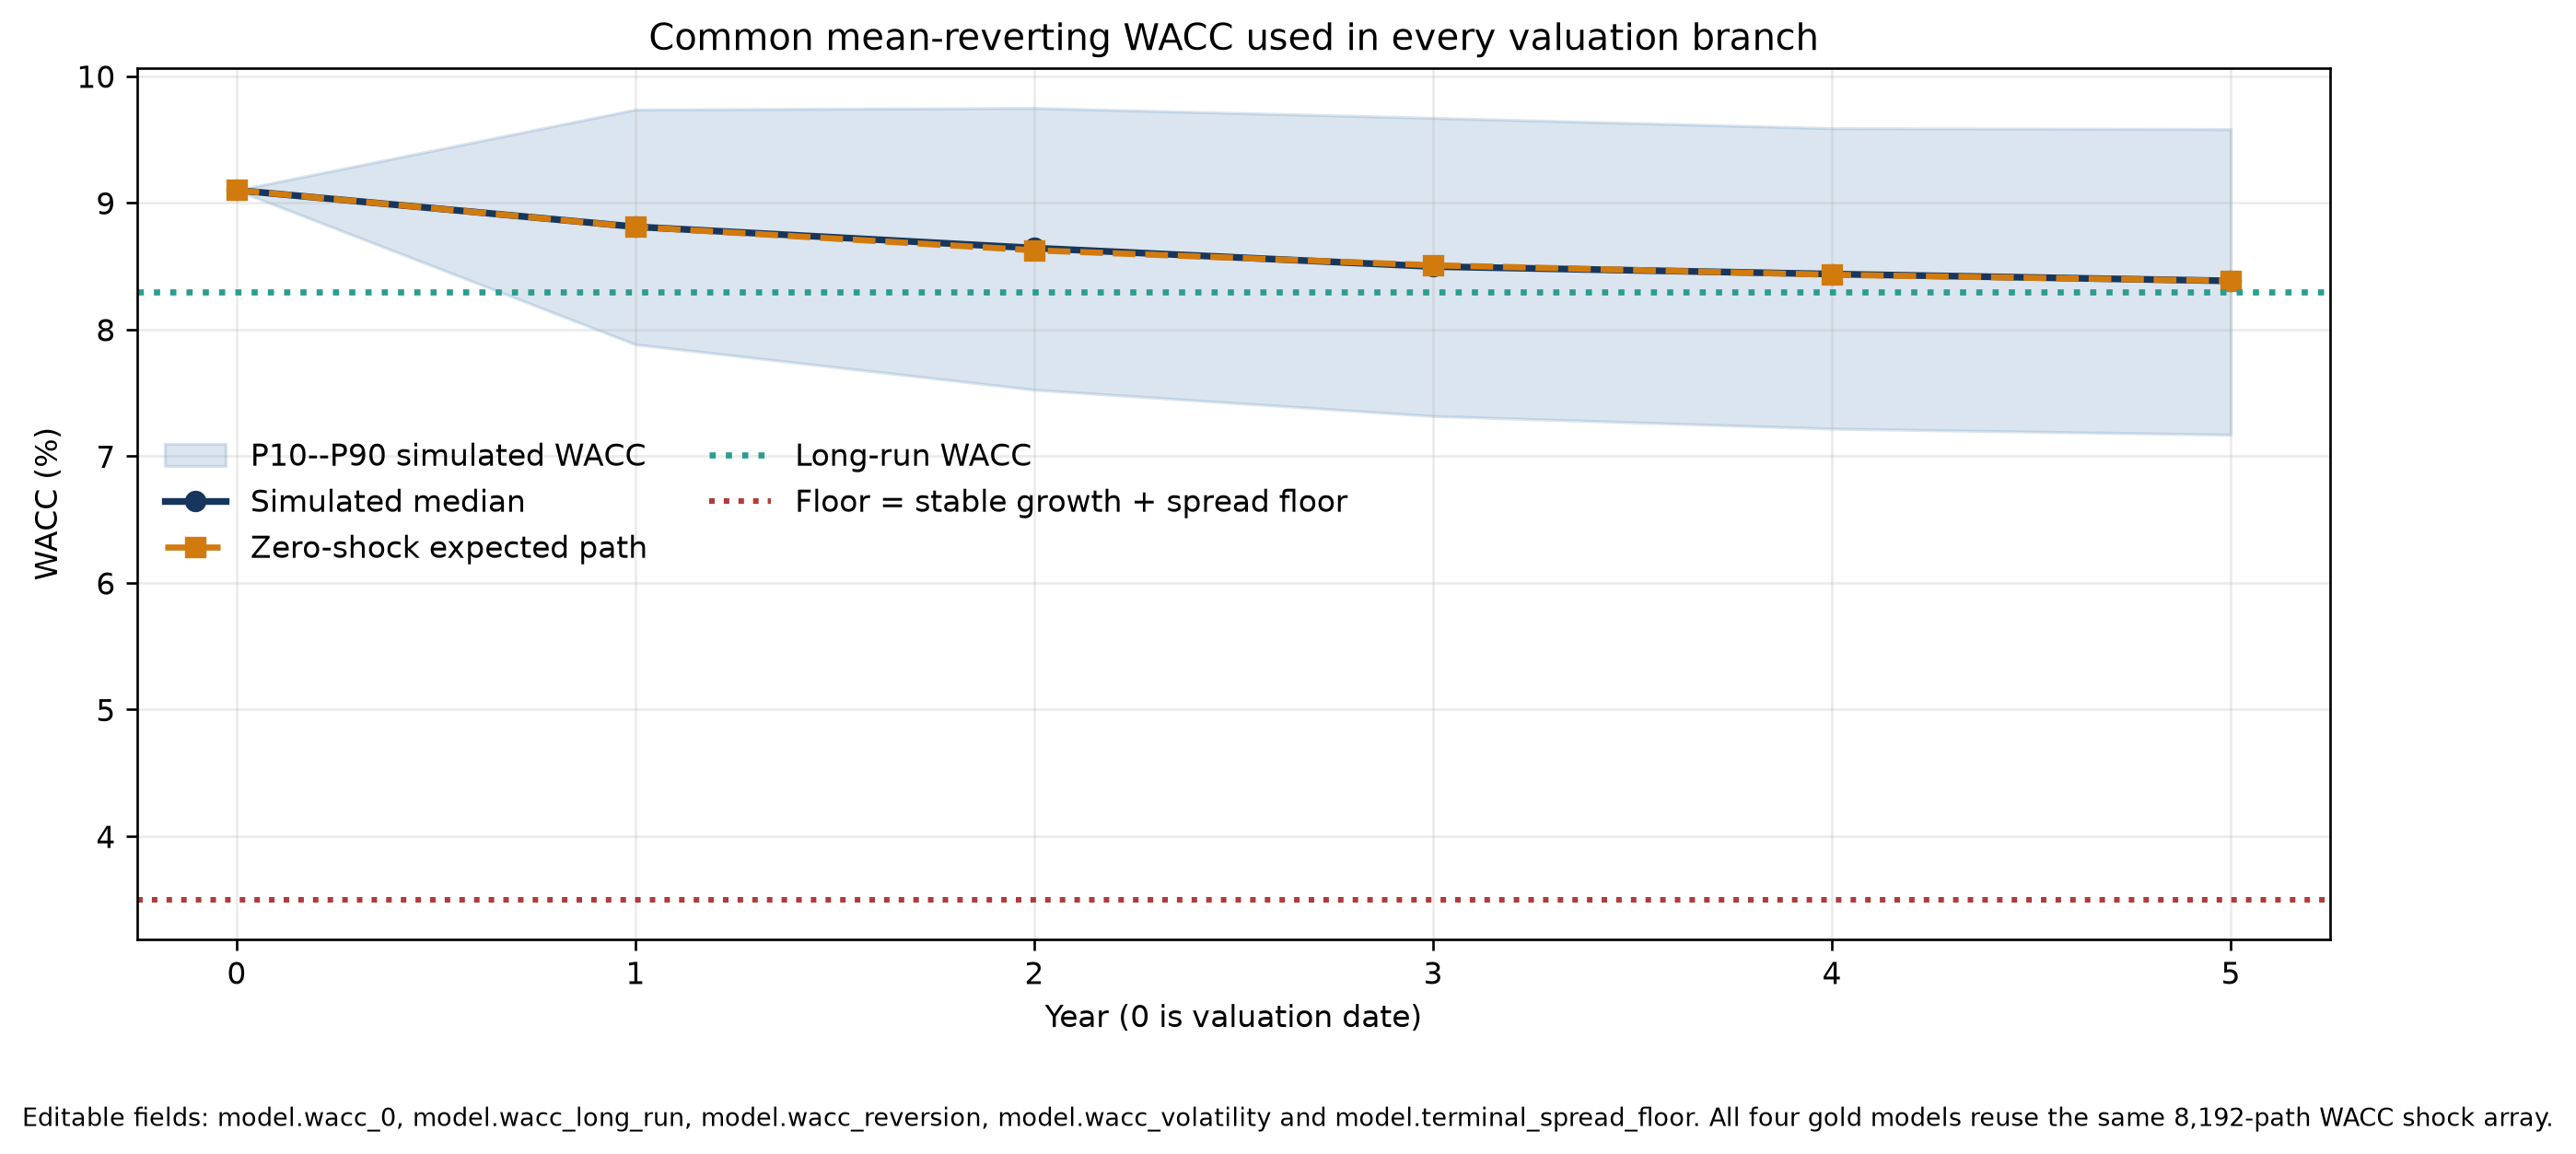
\includegraphics[width=0.95\columnwidth]{../img/publication/23df2023b1bd378f_fig_wacc_assumptions.png}
  \captionof{figure}{Common mean-reverting WACC. The band is the P10--P90 range from the shared 8,192-path shock array; the orange line is the zero-shock path and the dotted lines show the long-run level and admissibility floor.}
  \label{fig:wacc_assumptions}
\par}
\end{minipage}\par

\subsection{Terminal closure and sensitivity}
The terminal block uses $g_\infty=2.50\%$, $ROIC_\infty=10.50\%$ and terminal reinvestment of 23.81\%. At the median terminal WACC of \TerminalWACC\%, the terminal multiple is \TerminalMultiple$\times$ the final after-tax margin. The spread floor enforces $w_H>g_\infty$; \WACCClippedShare\% of simulated rates reach a clipping bound.

\noindent\begin{minipage}{\columnwidth}
{\centering
  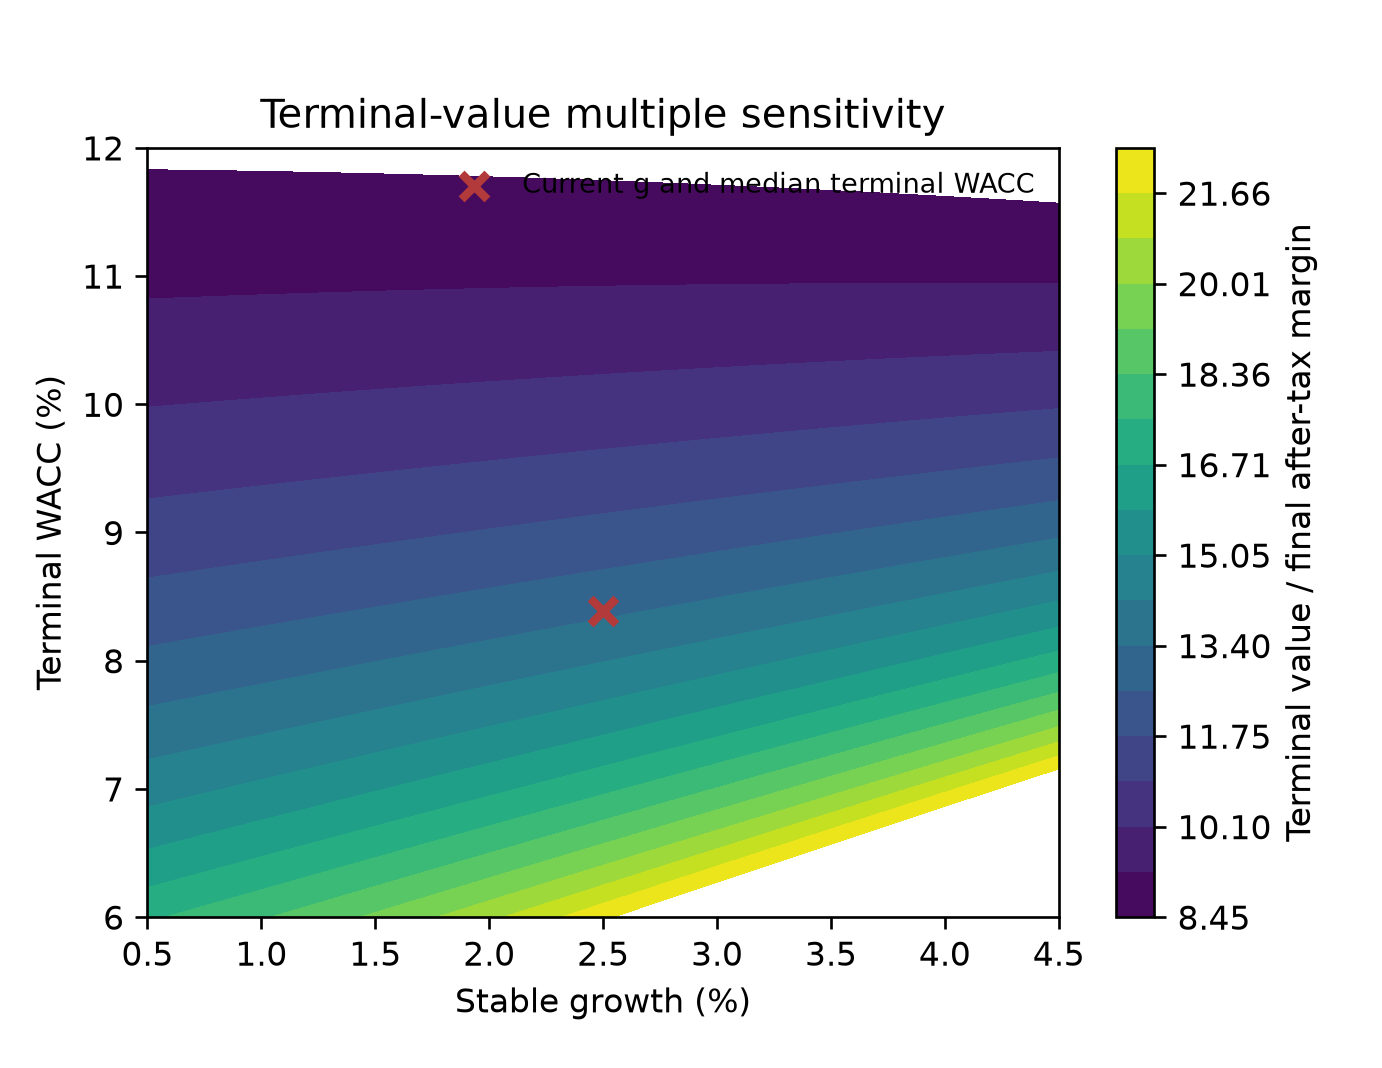
\includegraphics[width=0.90\linewidth]{../img/publication/2f2a7cea66301ac9_fig_terminal_multiple.png}
  \captionof{figure}{Terminal-value multiple sensitivity to stable growth and terminal WACC. The cross marks the configured stable-growth rate and current median terminal WACC.}
  \label{fig:terminal_value_mechanics}
\par}
\end{minipage}\par

\noindent\begin{minipage}{\columnwidth}
{\centering
  \includegraphics[width=0.90\linewidth]{\FigFigTerminalShare}
  \captionof*{figure}{\textbf{Figure~\ref{fig:terminal_value_mechanics} (continued).} Median proxy under the terminal conventions and with risk-free discounting of the explicit flows. Explicit flows to 2030 are worth about USD~11 billion against about USD~57--59 billion with a perpetuity. Zero terminal is a truncation scenario, not an estimated reserve life.}
\par}
\end{minipage}\par

\begin{table}[H]
\centering
\caption{Editable common DCF inputs.}
\label{tab:dcf_inputs}
\begin{tabularx}{\columnwidth}{@{}Xr@{}}
\toprule
Parameter & Value \\
\midrule
Tax rate & 25.00\% \\
$g_1\rightarrow g_\infty$ & 8.50--2.50\% \\
$ROIC_1\rightarrow ROIC_\infty$ & 14.50--10.50\% \\
$WACC_0\rightarrow\bar w$ & 9.10--8.30\% \\
WACC reversion & 0.45 \\
WACC volatility & 0.90\% \\
WACC floor/cap & 3.50/25.00\% \\
Terminal reinvestment & 23.81\% \\
\bottomrule
\end{tabularx}
\end{table}

\begin{methodbox}[Interpretation]
These are methodological assumptions, not filing-calibrated Barrick estimates. Terminal closure dominates the reported operating proxy: it accounts for about \TerminalShare\% of the mean. The former positive floor on the final margin is no longer used; it leaves medians unchanged.
\end{methodbox}

The quarterly bridge multiplies the average simulated gold price less unit Cost of Sales, both in USD per ounce, by production in thousand ounces, then divides by 1,000 to obtain component margin in USD millions. Each quarter is taxed, charged its reinvestment and discounted at its own date. This proxy is not reported EBIT or FCFF: production must be reconciled with sales and inventory, and depreciation, capital expenditure and working capital must enter without double counting. Fixed operating vectors exclude mine-level shocks and price-cost dependence.
